\begin{figure}[t]
\centering
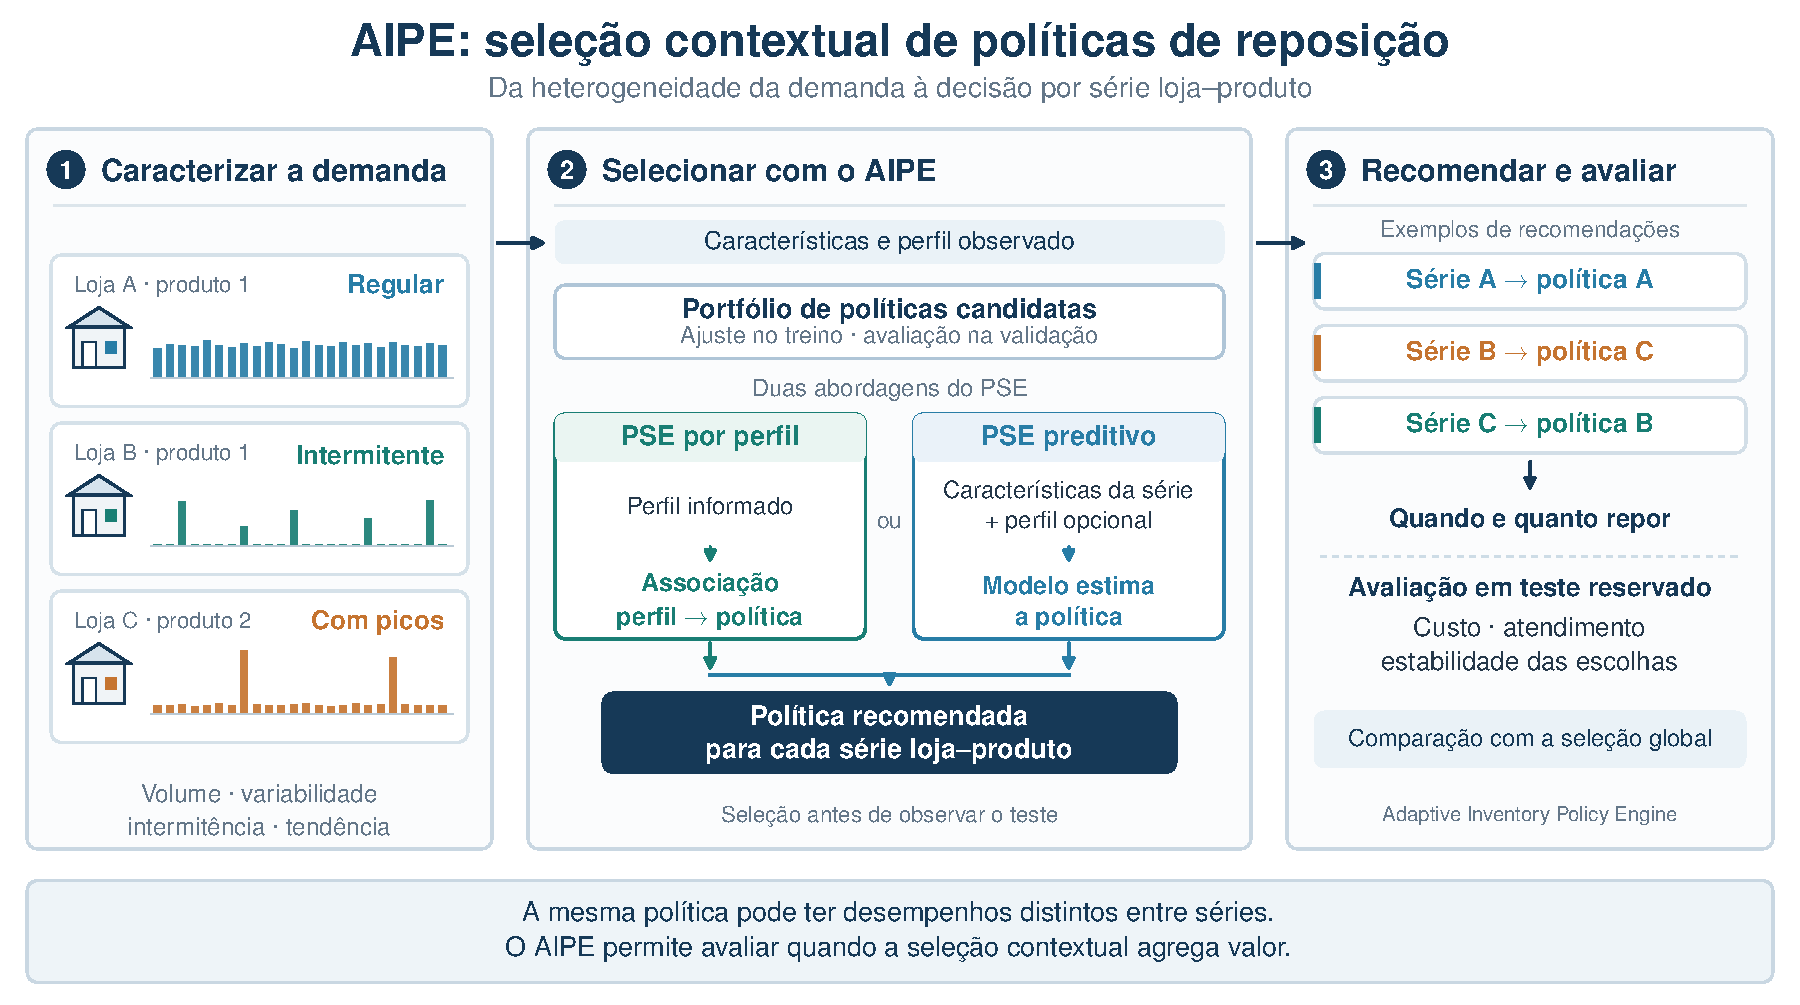
\includegraphics[width=\linewidth]{figures/aipe_conceito_v2_ptbr.pdf}
\caption{Visão conceitual do Adaptive Inventory Policy Engine (AIPE). Históricos heterogêneos são caracterizados por série loja--produto. O Policy Selection Engine (PSE) pode associar o perfil informado a uma política ou estimar a política a partir das características da série, com perfil opcional. As candidatas são ajustadas no treino e a seleção utiliza evidências de validação; custo, atendimento e estabilidade são avaliados no teste reservado, em comparação com a seleção global. Séries, políticas e associações são ilustrativas; a figura não representa resultados experimentais nem pressupõe superioridade da contextualização.}
\label{fig:aipe-conceito-v2}
\end{figure}
